\documentclass[11pt,oneside,a4paper,onecolumn]{report}
\usepackage{graphicx}
\usepackage{color}
\usepackage{setspace}
\usepackage{hyperref}
\usepackage{morefloats}
\usepackage{amsmath}
\usepackage{setspace}
\usepackage{subcaption}
\doublespacing
\usepackage[margin=1in]{geometry}
\setlength{\parindent}{20pt} % Do not automatically indent the paragraphs.

\newcommand{\SB}{SUPERball} %use \SB{} to write "SUPERball" correctly

\begin{document}

\title{DESIGN, BUILDING, AND TESTING OF SUPERball:\\ A TENSEGRITY ROBOT FOR SPACE EXPOLRATION}
\author{Jonathan Bruce}

\maketitle


% %%%%%%%%%%%%%%%%%%%%%%%%%%%%%%%%%%%%
% %%% Begin Table of Contents Page
% %%%%%%%%%%%%%%%%%%%%%%%%%%%%%%%%%%%%
% \renewcommand\contentsname{Table of Contents} % This command changes the name of the autogenerated table of contents (next line) from "Contents" to "Table of Contents".
% \tableofcontents % This command automatically generates the table of contents based on the sections in the document.
% \pagebreak[4]

% %%%%%%%%%%%%%%%%%%%%%%%%%%%%%%%%%%%%
% %%% End Table of Contents Page
% %%%%%%%%%%%%%%%%%%%%%%%%%%%%%%%%%%%%

% %%%%%%%%%%%%%%%%%%%%%%%%%%%%%%%%%%%%
% %%% Begin List of Figures Page
% %%%%%%%%%%%%%%%%%%%%%%%%%%%%%%%%%%%%

% \phantomsection % Create a phantom section such that the 'List of Figures' may be properly added to the table of contents.
% \addcontentsline{toc}{section}{List of Figures} % Add this section, 'List of Figures', to the table of contents.
% \listoffigures % This command automatically generates the list of figures based on the figures in the document.
% \pagebreak[4]

% %%%%%%%%%%%%%%%%%%%%%%%%%%%%%%%%%%%%
% %%% End List of Figures Page
% %%%%%%%%%%%%%%%%%%%%%%%%%%%%%%%%%%%%

% %%%%%%%%%%%%%%%%%%%%%%%%%%%%%%%%%%%%
% %%% Begin List of Tables Page
% %%%%%%%%%%%%%%%%%%%%%%%%%%%%%%%%%%%%

% \phantomsection % Create a phantom section such that the 'List of Tables' may be properly added to the table of contents.
% \addcontentsline{toc}{section}{List of Tables} % Add this section, 'List of Tables', to the table of contents.
% \listoftables % This command automatically generates the list of tables based on tables in the document.
% \pagebreak[4]

% %%%%%%%%%%%%%%%%%%%%%%%%%%%%%%%%%%%%
% %%% End List of Tables Page
% %%%%%%%%%%%%%%%%%%%%%%%%%%%%%%%%%%%%

\copyrightpage

\tableofcontents

\listoffigures

\listoftables

\begin{abstract}
Presented in this work are the concepts to build, sense and control a completely untethered tensegrity robotic system called \SB{} (Spherical Underactuated Planetary Exploration Robot), which is a compliant icosahedron tensegrity robot designed to enable research into tensegrity robots for planetary landing and exploration as part of a NASA funded program.
Tensegrity robots are structurally compliant machines, uniquely able to absorb forces and interact with unstructured environments through the use of multiple rigid bodies stabilized by a network of cables.
However, instead of engineering a single new robot, a fundamentally reusable component for tensegrity robots was developed by creating a modular tensegrity robotic strut which contains an integrated system of power, sensing, actuation, and communications.
\SB{} utilizes six of these modular struts, making the \SB{} system analogous to a swarm of 6 individual robots, mutually constrained by a cable network.

Since \SB{} is intended for use on planetary surfaces without the support of GPS, state estimation and control policies only utilize the sensors on board the robotic system.
When external sensors are used, they must be able to account for imprecise placement and automatic calibration.
Also, dynamic tensegrity systems do not exhibit continuous dynamics due to nonlinear cable conditions and interactions with the environment, thus non-traditional control development methods are implemented.
In this work, control polices are developed using Monte Carlo, evolutionary algorithms, and advanced supervised learning through Guided Policy Search.
Each system is evaluated in simulation, while state estimation and the Guided Policy Search method are additionally evaluated on the physical \SB{} robotic system.
\end{abstract}

\begin{dedication}
\vspace*{\fill}
\begin{center}
A loving dedication.
\end{center}
\vspace*{\fill}
\end{dedication}

\begin{acknowledgements}
Proper acknowledgments of everyone else who helped you graduate.

The text of this thesis includes reprints of the following previously published
material: \cite{NIACfinalreport, Vytas_IPPW_2013, bruce2014design, sabelhaus2015system, caluwaerts2016esitmation, geng2016deep}

\end{acknowledgements}

\chapter{Introduction}

As part of our research for the NASA Innovative Advanced
Concepts  (NIAC)  program,  we  are  developing  the  SUPER-
ball (Spherical Underactuated Planetary Exploration Robot),
which is a compliant icosahedron tensegrity robot designed
for   planetary   landing   and   exploration.   Tensegrity   robots
are  soft  machines  which  are  uniquely  able  to  compliantly
absorb  forces  and  interact  with  unstructured  environments.
However, instead of engineering a single new robot, we have
chosen  to  develop  a  fundamentally  reusable  component  for
tensegrity  robots  by  creating  a  modular  robotic  tensegrity
strut which contains an integrated system of power, sensing,
actuation, and communications. The purpose is to enable the
exploration of the wide range of possible tensegrity robotic
morphologies  by  simply  combining  the  robotic  struts  into
new systems.

It is possible to design free-standing structures by arrang-
ing  axially  loaded  compression  elements  in  a  well  crafted
network of tensional elements. Such an arrangement is called
a tensegrity structure (tensile integrity). Each element of the
structure  experiences  either  pure  axial  compression  or  pure
tension [1][2]. The absence of bending or shear forces allows
for highly efficient use of materials, resulting in lightweight,
yet robust systems.
Because the struts are not directly connected, tensegrities
have  the  unique  property  that  externally  applied  forces  dis-
tribute  through  the  structure  via  multiple  load  paths.  This
creates  a  soft  structure,  for  a  soft  robot,  out  of  inherently
rigid  materials.  Since  there  are  no  rigid  connections  within
the structure, there are also no lever arms to magnify forces.
The  result  is  a  global  level  of  robustness  and  tolerance  to
forces applied from any direction.
This  makes  tensegrity  robots  inherently  compliant  and
extremely well suited for physical interactions with complex
and  poorly  modeled  natural  environments.  Active  motion
in  tensegrity  robots  can  be  performed  by  changing  cable
lengths in parallel, enabling the use of many small actuators
that  work  together,  rather  than  individual  heavy  actuators
which   work   in   series.   There   are   also   many   indications
that tensegrity properties are prevalent throughout biological
systems,  and  the  morphology  of  the  SUPERball  that  we
are  studying,  especially  when  carrying  a  payload,  ends  up
bearing  a  striking  resemblance  to  the  nucleated  tensegrity
model of cell structure.

Because  of  the  limited  research  into  actuated  tensegrity
robotics,   many   design   aspects   have   yet   to   be   carefully
studied. To date, the majority of constructed tensegrity robots
have  been  simple  prototypes  using  servo  motors,  limited
sensing,  and  are  often  tethered  for  power  and  control  [5].
Others have had fewer limbs than the SUPER ball, or have
been  secured  to  the  ground  as  opposed  to  free-standing
[6][7]. Some related approaches utilize tensegrity as part of a
larger, more complicated system, but not as the primary loco-
motion method [8]. Others have created designs that do not
use direct cable actuation, as in the SUPER ball, but instead
have  more  limited  forms  of  locomotion  through  vibration
[9][10]. Finally, the most similar designs to the SUPER ball
have not been engineered to specific design requirements nor
have  the  advanced  sensing  framework  needed  for  controls
testing [11]

The  high  strength-to-weight  ratio  of  tensegrity  structures
is very attractive due to the impact of mass on mission launch
costs.  Large  tensegrity  structures  have  been  shown  to  be
deployable from small compact configurations which enable
them to fit into space constrained launch fairings. While the
above qualities have inspired studies of deployable antennae
and  other  large  space  structures  [12],  it  is  in  the  realm
of  planetary  exploration  that  we  see  the  most  significant
role  for  many  of  the  unique  force  distribution  qualities  of
tensegrity  robots.  A  recent  NIAC  project  [13]  specifically
studies  landing  and  surface  mobility  of  tensegrities,  ex-
ploiting  the  controllable  compliance  and  force  distribution
properties which make for reliable and robust environmental
interactions.
The   main   goal   is   to   develop   tensegrity   probes   with
an  actively  controllable  tensile  network  to  enable  compact
stowage  for  launch,  followed  by  deployment  in  preparation
for  landing.  Due  to  their  natural  compliance  and  structural
force  distribution  properties,  tensegrity  probes  can  safely
absorb significant impact forces, enabling high speed Entry,
Descent, and Landing (EDL) scenarios where the probe itself
acts  much  like  an  airbag.  However,  unlike  an  airbag  which
must  be  discarded  after  a  single  use,  the  tensegrity  probe
can  actively  control  its  shape  to  provide  compliant  rolling
mobility  while  still  maintaining  the  ability  to  safely  absorb
impact  shocks  that  might  occur  during  exploration.  This
combination  of  functions  from  a  single  structure  enables
compact and lightweight planetary exploration missions with
the capabilities of traditional wheeled rovers, but with a mass
and cost similar or less than a stationary probe.

Therefore, a large fraction of the overall weight (as mea-
sured  at  atmospheric  entry)  of  a  tensegrity  mission  can  be
used  for  the  scientific  payload  due  to  the  dual  use  of  the
structure  as  a  lander  and  a  rover.  This  allows  for  cheaper
missions  and  enable  new  forms  of  surface  exploration  that
utilize the natural tolerance to impacts of tensegrities [14].

Buckminster Fuller [1] and the artist Kenneth Snelson [2]
initially  explored  tensegrity  structures  in  the  1960s.  Until
the  mid-1990s  the  majority  of  tensegrity  related  research
was  concerned  with  form-finding  [15]  and  design  analysis
of  static  structure  [16][17].  More  recently,  active  control
efforts  for  tensegrities  began  to  emerge  [18],  as  well  as
descriptions  of  the  dynamics  of  tensegrity  structures  taking
the connectivity pattern into account [17].
The tensegrity principle allows for compliance and multi-
path load distribution, which is ideal for physical interaction
with  the  environment.  However,  these  aspects  also  present
significant  challenges  to  traditional  control  approaches.  A
recent  review  [19]  shows  that  there  are  still  many  open
problems in actively controlling tensegrities, especially when
interacting  with  an  environment  during  locomotion  or  ma-
nipulation  tasks.  Though  work  has  been  done  to  control  a
tensegrity  to  change  into  a  specified  shape  [20],  practical
determination  of  the  desired  shape  itself  is  an  ongoing
challenge.  Recently,  locomotion  of  icosahedral  tensegrity
robots  through  body  deformation  was  demonstrated  [21].
Other work has addressed collision between rigid tensegrity
elements during control generation [22][23].
The  approach  taken  by  the  NASA  Dynamic  Tensegrity
Robotics  Lab  builds  on  this  by  developing  body  defor-
mation  control  algorithms  based  on  central  pattern  gen-
erators  [24][25],  distributed  learning,  reservoir  computing,
and  genetic  algorithms  [26],  instead  of  traditional  linear
and  nonlinear  systems  approaches.  To  date,  our  approach
has  shown  promising  results  at  productively  harnessing  the
potential  of  complex,  compliant,  and  nonlinear  tensegrity
structures.

\section{Motivation}

Though there is much prior work in a variety of theoretical
areas for tensegrities, engineering knowledge of constructing
practical  tensegrity  robots  is  limited.  Since  a  staggering
variety  of  different  tensegrity  structures  can  be  constructed
from  collections  of  simple  sticks  and  strings  (for  example,
see the TensegriToy modeling kit), we have made it a priority
to develop self-contained robotic tensegrity struts which can
be  used  to  explore  and  build  a  wide  range  of  tensegrity
robots  simply  by  combining  them  into  novel  structures.
Our  designs  are  driven  by  experimental  results  obtained
from  a  previous  prototype,  ReCTeR  (Reservoir  Compliant
Tensegrity Robot) in combination with simulation results of
our validated tensegrity simulator NTRT (NASA Tensegrity
Robotics Toolkit) [27][28]

\section{Application}


\section{Goal}

In  order  to  develop  SUPERball  from  ReCTeR’s  design
limitations as well as our lab’s need for rapid experimentation
of  various  tensegrity  configurations  and  morphologies,  we
came  up  with  a  modular  tensegrity  platform  to  research
large  scale  robotic  tasks;  e.g.  a  tensegrity  planetary  probe
to explore Saturn’s moon Titan.
A.  Design Requirements
Our lab obtained design requirements through an iterative
approach  involving  NTRT  and  ReCTeR.  As  we  recently
validated  our  NTRT  simulator  by  experimental  validation
with  ReCTeR  [28],  we  can  now  quickly  evaluate  various
tensegrity  configurations  in  simulation  to  find  optimal  me-
chanical  design  goals.  Next  to  the  NTRT  solver,  we  also
incorporated  results  obtained  with  our  (open  source)  Euler
Lagrange solver based on Skelton’s work [17] and measure-
ments on ReCTeR.
The design requirements obtained from the NTRT simula-
tions are given in Table I. We are confident that a tensegrity
robot achieving the following conditions will be capable of
dynamic locomotion, as shown by our evaluation of control
policies in Section V.


\chapter{Mechatronic Design}

An ideal tensegrity system, either robotic or static, is a collection of rigid compressible elements suspended within a network of tensioned cables where non of the compressible elements are in direct contact with one another. 
For a robotic tensegrities without a payload, the actuation and supporting electronics would be logically designed into the compressible elements. 
For the inception of \SB{}, this compressible element was further dissected into three parts: two identical end caps (Modular Tensegrity Robots) and a section of tube stock.


%For \SB{}, the idea of making the compressible element  a self contained module that could be the coupled with another identical module  

%For SUPERball, each compressible element would be comprised of three parts: two identical end caps and a piece of tube stock. 
%Therefore, SUPERball can be thought of as a collection of identical robots (end caps) connected mechanically through rods and cables to enable entire system the ability to locomote.
%In this section, the main focus will be the mechatronic description of the end cap, with a focus on how each subsystem was designed to achieve an unteathered tensegrity for locomotion and system state research. 



\begin{figure}[thpb]
\begin{subfigure}{.5\textwidth}
      \centering
      \includegraphics[width=0.5\columnwidth]{tex/img/endcap_upclose_sensorboard_labelled_fixedfonts}
      \caption{end cap front side.}
      \label{fig:endcap_upclose_front}
\end{subfigure}
\begin{subfigure}{.5\textwidth}
      \centering
      \includegraphics[width=0.5\columnwidth]{tex/img/endcap_upclose_motorboard_labelled_fixedfonts}
      \caption{end cap back side.}
      \label{fig:endcap_upclose_back}
\end{subfigure}
\caption{Fully assembled end cap images on SUPERball}
\label{fig:fully_assembled_endcap}
\end{figure}

\section{Mechanical}
Write about the mechanical design of SUPERball. Make sure to give credit where credit is due.

B.  Mechanical Design
The main structural elements of the end caps were
kept as  simple as possible and  in  sections  to  enable  each  end  cap  to  be self  contained  so  that  the  end  cap  may be removed from the connecting rod as one whole unit.
The end  caps  are  held  onto  the  connecting  rods  by  a  simple tube  collar  for  easy  removal. 
There  are  5  sections  to end cap: a spring holder, battery holder, motor and electronics, cable actuation and routing, and a ground contact. 
These sections as they are designed for SUPERball are shown in figure \ref{}. 
Design parameters, both ideal goals and built, are shown in table \ref{} **Table with design parameters!!**
For simplicity in manufacturing, the supporting structure is made from bent 6061-T6 aluminum sheet unless otherwise noted.

\subsection{Spring Holder}
A  lesson  learned  from other tensegrity robots and the designer of ReCTeR (reference) was  that  externally  exposed springs are not ideal for a robotic system that would be interacting with a dynamic and unknown enviroment. 
The exposed springs get caught on objects and the assumption of near mass-less cables  can  no  longer  be  applied.  
On  the  end  cap for SUPERball, an enclosed compression spring system was developed  to  alleviate  these  issues.  
Compression  springs were chosen so that during any unknown impact, the springs would not plastically deform without the need for any external hardware. 
For SUPERball, a spring with a spring constant of \(998 Nm\) is attached to a passive cable element  and  a \(2850 Nm\) spring  is  attached  to  an  actuated cable.  
A  passive  spring was chosen with a total throw of \(23 cm\) to allow for pretension to be instated into the passive springs as well as to allow a wide dynamic compliant range.  
Since the cables which are actuated will be able to dynamically control the pretension, a smaller throw spring was chosen to conserve space.

\subsection{Battery Holder}
\label{battery_holder}
From the inception of SUPERball, enabling a self-contained power source which was easily accessible per end cap was a driving design parameter.
During the initial design and build of SUPERball, It was known that the batteries where to be 24 volt lithium polymer but optimal size and shape of the battery was unknown due to a changing power profile.
Therefore, a battery holder with a simple securing mechanism which can handle a wide range of battery sizes was utilized.
Two hook and loop straps where used with simple slot cutouts to enable cinching around a generic lithium polymer battery.
The holder was also made large enough to hold the Power Board PCB board opposite of the battery.
As shown in section \ref{power_board}, the Power Board was designed to be an low profile to allow for a large battery within the holder.
Figure \ref{}**reference a picture of just the battery holder** shows a the battery holder as designed on SUPERball.

\subsection{Motor and Electronics}
\label{mechanical:motor}
This section of SUPERball was mechanically designed around the Maxon EC-22 100 watt BLDC motor used for actuation. 
Each Maxon motor is \(22 mm\) in diameter and \(108 mm\) long with gearbox and encoder.
The output shaft is a \(6 mm\) in diameter D shaft of length \(10.2 mm\).
A size requirement for how large the cross sectional diameter of the end cap could be was quite a limiting factor in designing the motor and electronic section.
The maximum diameter for any section used in the end cap was maximally limited to double the diameter of the connecting rod.
The idea for such a limitation was to keep the effective moment arm out from the center axis of any rod to a minimum.  
Due to the spring size and the need for a spring holder tube, the minimum diameter for the connecting rod was \(~35mm\) giving a maximum end cap diameter of \(70mm\).

The main component in the motor and electronic section of the end cap, is the cable routing support bracket. 
This bracket plays three roles in the mechanical design: static support for the motor, support for the supporting material, and main exit support for the internal cable routing.
Figure \ref{} **figure of the cable routing supporting bracket** shows the cable routing support bracket.
The actual motor mount was designed to be mechanically floating to enable torque sensing directly on the motor mount.
Thus, the cable routing support bracket sinks the reaction torque induced by the motor.
The motor mount bracket with torque sensor can be seen in figure \ref{}.
There are two electronic boards, the Sensor and Motor boards, which are mounted to brackets that straddle the motor.
Due to space limitations, these brackets are also load bearing components for the torsional forces induced by the motor.
Figure \ref{} **reference the main figure for the end cap** shows one of the brackets with the corresponding electronic board mounted.

\subsection{Cable Actuation and Routing}
A simple spool design was implemented to directly actuate the cable. 
The spool directly couples to the motor shaft by press fitting onto the D shaft.
The force vector applied to the spool by the actuated cable will never be perpendicular to the spool, therefore a thrust bearing was embedded into the spool and a radial bearing supports the top of the spool.
For completeness, spool has the ability to slide along the the shaft's main axis and the thrust bearing sinks the trust force into the motor mount.
Since this thrust force is perpendicular to the torque of the motor, this force is not induced into the torque sensor built into the motor mount.
Figure \ref{} shows the spool with thrust bearing cutout and radial bearing.

There are three other cables that connect to an end cap.
Two are routed through the end cap to the spring housing section and the other is terminated on the end cap.
The cables used externally from the end cap is composed of Vectran braided cable and the cables used within the end cap are braided steel cabling. 
Both routed cables enter the end cap through the cable routing support bracket mentioned in \ref{mechanical:motor}.
The cables are immediately routed around a rolling guide bearing to induce an approximate 90 degree bend to guide the cables towards the spring tube holder section.
After the rolling guide bearing, the cables enter a PTFE tube to create a type of bowden cable to help route the cables around components within the end cap.
Once the cables reach their respective spring within the spring tube holder, the PTFE tube is terminated and the cable is routed through the spring and terminated using a copper compression sleeve.

\subsection{Ground Contact} 
This final section of the end cap is the simplest. 
To protect the end cap during locomotion, a 3D printed cap was manufactured to cover the end.
This part is designed so that it is the only part of the end cap that contacts the ground during normal locomotion.
To decrease the impact shocks as the rod contacts a surface, compliant foam sheets are place between the 3D printed cap and the end cap.
Figure \ref{} shows the 3D printed cap and the foam sheets.

\section{Electrical}
\SB{}'s electronics where developed with a focus on reliability, safety, and enabling distributed controls.
Another parameter was the ability to drive the 100W BLDC Maxon motors (see section \ref{mechanical:motor} for detailed information on this motor).
These main design criteria gave way to implement separate electronic boards per end cap based on their main function.
Each end cap has three custom Microchip dspic33e enabled PCB boards and only one end cap per rod has an ARM based computer called a Beagle Bone Black.
Each custom PCB is designed for very different purposes: A board to condition sensor data and run real-time control loops, a board to condition and distribute a 5.5V electronic power rail and a 24V motor power rail, and a board to control the 100W BLDC motor. 
The only requirements for each custom board is full CAN bus communication and power conditioning required for the 5.5V power rail.
The boards are simply named by their main purpose, thus Sensor, Power, and Motor respectively.

\subsection{Motor Board}
An initial driving parameter used during the design of SUPERball was the BLDC motor. 
During the design review for \SB{}, a lightweight motor with high power and efficiency was wanted.
Thus, a Maxon brushless motor was a logical choice (see section \ref{mechanical:motor} for detailed information on this motor).
In order to effectively drive this motor, a dedicated motor board was used on each end cap.
The main development of this board was engineered by Pavlo Manovi, and certain aspects of the board where tailored for our needs \ref{}.
The main components on the Motor board are the Microchip's 16-bit dsPIC33ep256mu506 micro-controller and the Texas Instruments DRV8303 three phase pre-driver.
Figure \ref{} shows the current version of the motor board.

\subsection{Sensor Board and Beagle Bone Black}
\label{sensor_bbb}
The sensor board was originally designed as the main processing unit on an end cap for \SB{}. 
However, the design and building process has lead to the coupling of the sensor board with a Beagle Bone Black.
For a detailed explanation of why the Beagle Bone Black was integrated into the system, please refer to \ref{communication}.

The current version of the sensor board was developed as a daughter board for Beagle Bone Black \ref{}.
The board mates to the Beagle Bone Black through two double row 46 pin headers and provides power and CAN communication to the ARM board.
The main processing unit on the sensor board is Microchip's 16-bit dsPIC33ep128gp506 micro-controller.
Environmental sensing is enabled through a 9DOF inertial measurement unit (IMU) and a 24-bit analog to digital converter (ADC) configured in a half wheat-stone bridge configuration.
The IMU is comprised of Invensense's MPU6000 mastered to Freescale's MAG3110 magnetometer, and the ADC is Analog Device's AD7193.

The Beagle Bone Black is a open-source hardware single-board computer inspired by the BealgBoard, the larger predecessor developed by Texas Instruments as an educational tool.
The main processor on the board is a Sitara ARM Cortex-A8 processor running at 1Ghz and capable of running a full ARM based operating system.
The processor is also able to interface directly with low level communication protocols such as CAN, UART, SPI, and I2C.
To meet our memory and speed requirements, a custom kernel was built with only the main modules needed by our system.
On top of this kernel, the Beagle Bone Black is running a ROS (Robot Operating System, see section \ref{communication} for more detials) enabled Ubuntu ARM 14.04.1 LTS operating system.

A new feature still being developed is the integration of DecaWave's DWM1000 module for relative distance measurements.
Legacy components no longer utilized on the sensor board are mounting pins for an XBee device.
A small breakout was designed to integrate the DWM1000 module into where the XBee device was originally mounted.
Figure \ref{} shows the sensor board mounted to a Beagle Bone Black and the DWM1000 module.

\subsection{Power Board}
\label{power_board}
The power board was design to enable safety, both for a person working near \SB{} and for the electronics, as well as conditioning input power to both a 5.5V and a 24V rail.
The board was also designed with a minimal height profile allowing for larger batteries to be placed near the board.
See section \ref{battery_holder}, to view the section which houses the power board.
The main idea of safety is focused around operating the 100W BLDC motors, thus a two battery system was implemented.
A small battery used for starting the micro-controller boards but not capable of producing 24V needed by the motor, and a large battery used during main operation of the end cap.
The two batteries used are a 160 milli-amp-hour 1-cell and a 3 amp-hour 6-cell lithium polymer batteries, named the back-up and the main receptively.
To enable the 24V power, multiple input conditions should be met fed into an analog and-gate.
The input conditions are: a physical switch located on the end cap, a digital logic pin from the power board's micro-controller, power being applied by the back-up battery, and a signal coming from a dedicated 8-bit micro-controller monitoring a pulsed wireless 2.4Ghz signal.
If any one of these conditions go false, then the full 24V rail is disabled.
There are also fuses on both the 24V and 5.5V line to protect all the micro-controller circuits from shorts.
Figure \ref{fig:connection_diagram} shows a basic connection diagram for the power lines.

The main processing unit on the power board is Microchip's 16-bit dspicPIC33ep128mc506 mirco-controller.
The wireless "kill switch" monitoring mirco-controller is Mircochip's 8-bit PIC12(L)F1571/2 mirco-controller.
This chip monitors a known pulse width being communicated by a Nordic Semiconductor nRF24L01 breakout board with antenna.
The pulsed signal is sent by a hand held unit off the robot.
When a shut off command is sent or the PIC12's watchdog timer is triggered from a delay in wireless signal, the logic signal sent from the PIC12 is turned to false disabling the 24V power rail. 
5.5V power is either supplied by the back-up battery or the main battery using a custom boost or buck switching circuit, receptively.
The 24V rail is supplied directly from the main battery when all input logic is enabled.
Figure \ref{} shows the power board with nRF24l01 chip mounted. 

\section{Communication and Power}
\label{communication}

Communication on \SB{} was designed around a desire to have each rod of the tensegrity system unteathered from any other part of the system.
Two wireless protocols as well as a wired Controller Area Network, or CAN, bus were implemented.
The two main wireless protocols are WiFi for main data communication and a 2.4GHz channel for wireless switching power for safety.
Figure \ref{fig:connection_diagram} shows how power and communication are connected for a single end cap and figure \ref{fig:ros_diagram} shows the connections for \SB{}'s wireless communications.

\begin{figure}[thpb]%{.5\textwidth}
      \centering
      \includegraphics[width=0.8\columnwidth]{tex/img/hard_wire_connection}
      \caption{This is a connection diagram for power and communication for an end cap on \SB{}.}
      %\vspace{-0.5cm}
      \label{fig:connection_diagram}
\end{figure}

\subsection{CAN Bus}
A communication design was desired that would be robust, extensible, and work over long distances.
A CAN bus fits these main requirements and was implemented to be the main communication between all controllers on a single rod.
Since the CAN bus is a physical layer standard, a communication protocol is usually required to get a robust and extensible network.
A widely accepted protocol that has been well tested and understood, is the CANOpen protocol \ref{}.
CANOpen defines the addressing scheme, several small communication protocols and an application layer defined by a device profile.
Some of the smaller communication protocols supported by CANOpen are device monitoring and communication between nodes, network management, and a simple transport layer for message processing.
This open source protocol is freely distributed and has many open and closed source implementations.
The CANOpen implementation used for \SB{} is the CANFestival project which focuses on implementing the basic protocol while maintaining a small code base and low computational load for embedded systems \ref{}.
Each mirco-controller and Bealge Bone Black are able to run the entire CANFestival project code in less than \(150 \mu s\) under worst case scenarios.
The physical layer CAN bus is running at \(1 Mbit/s\) 

\subsection{WiFi and the Robot Operating System}
The Robot Operating System, or ROS, is a collection of software to provide operating system functionality on a network linked computer cluster. 
Message-passing and packet management works agnostic to the network layer, allowing information to be passed from one ROS enabled node to any other ROS enabled node on a network.
Figure \ref{fig:ros_diagram} shows a basic representation of how this message-passing works on the \SB{} ROS network.

As explained in section \ref{sensor_bbb}, enabling each rod is a ROS node was the driving reason to have at least one ARM based chip on every rod.
Since the Beagle Bone Black is also on the CAN bus, it's main function is to sniff the CAN network and send new information out to the ROS network.
This enables for near real time data analysis and for time stamped data logging on \SB{}.

\begin{figure}[thpb]%{.5\textwidth}
      \centering
      \includegraphics[width=0.8\columnwidth]{tex/img/ROS_Wireless}
      \caption{A simplified representation of how messages are passed within the \SB{} ROS network.}
      %\vspace{-0.5cm}
      \label{fig:ros_diagram}
\end{figure}

%\chapter{Modeling and Model Validation}
\label{modeling}

\begin{figure}[thpb]
      \centering
      \includegraphics[width=0.8\columnwidth]{tex/img/superball_roverscape2_cropped.jpg}
      \caption{SUPERball, fully assembled, in the NASA Ames Research Center Roverscape.}
      \label{fig:SB}
\end{figure}

As part of our research for the NASA Innovative Advanced
Concepts  (NIAC)  program,  we  are  developing  the \SB{} (Spherical Underactuated Planetary Exploration Robot),
which is a compliant icosahedron tensegrity robot designed
for   planetary   landing   and   exploration, seen in figure \ref{fig:SB}.   Tensegrity   robots
are  soft  machines  which  are  uniquely  able  to  compliantly
absorb  forces  and  interact  with  unstructured  environments.
However, instead of engineering a single new robot, we have
chosen  to  develop  a  fundamentally  reusable  component  for
tensegrity  robots  by  creating  a  modular  robotic  tensegrity
strut which contains an integrated system of power, sensing,
actuation, and communications. The purpose is to enable the
exploration of the wide range of possible tensegrity robotic
morphologies  by  simply  combining  the  robotic  struts  into
new systems.

Though there is much prior work in a variety of theoretical
areas for tensegrities, engineering knowledge of constructing
practical  tensegrity  robots  is  limited.  Since  a  staggering
variety  of  different  tensegrity  structures  can  be  constructed
from  collections  of  simple  sticks  and  strings, we have made it a priority
to develop self-contained robotic tensegrity struts which can
be  used  to  explore  and  build  a  wide  range  of  tensegrity
robots  simply  by  combining  them  into  novel  structures.
Our  designs  are  driven  by  experimental  results  obtained
from  a  previous  prototype,  ReCTeR  (Reservoir  Compliant
Tensegrity Robot) in combination with simulation results of
our validated tensegrity simulator NTRT (NASA Tensegrity
Robotics Toolkit)~\cite{2917079}\cite{Caluwaerts2013rsif}.

In  order  to  develop  SUPERball  from  ReCTeR's  design
limitations as well as our lab’s need for rapid experimentation
of  various  tensegrity  configurations  and  morphologies,  we
came  up  with  a  modular  tensegrity  platform  to  research
large  scale  robotic  tasks;  e.g.  a  tensegrity  planetary  probe
to explore Saturn's moon Titan.
%Our lab obtained design requirements through an iterative
%approach  involving  NTRT  and  ReCTeR.  As  we  validated  our  NTRT  simulator  by  experimental  validation
%with  ReCTeR~\cite{Caluwaerts2013rsif} and can  now  quickly  evaluate  various
Our lab obtained design requirements through an iterative approach with validated our NTRT simulator by experimental comparison with ReCTeR~\cite{Caluwaerts2013rsif}.
We now can quickly  evaluate  various
tensegrity  configurations  in  simulation  to  find  optimal  mechanical  design  goals.  In conjunction with the  NTRT  solver,  we  also
incorporated  results  obtained  with  our  (open  source)  Euler
Lagrange solver based on Skelton's work~\cite{Skelton2009} and measurements on ReCTeR.
The initial design requirements obtained from the NTRT simulations, refined designs after a first prototype build, and how these compare to other tensegrity robotic systems are given in Table \ref{design_req}.


\begin{table*}[ht]
%\begin{minipage}[t][\linewidth]{
\caption{\SB{} and Related Robots Design Overview.} 
\label{design_req}

\begin{center}%
\resizebox{\columnwidth}{!}{%
\begin{tabular}{lrrrcrrrrrrr}
%\hline
&$\bm{l_{strut}}$ & $\bm{\Delta l_{act}}$ & $\bm{k_{passive}}$ & \bf{tethered?} & \bf{control} & $\bm{f_{act}}$ & \bf{\#act.} & \bf{mass} & \bf{sensors} &\bf{actuators} &\bf{ref.} \\ \hline \hline
\bf{Pneumatic}&\SI{.57}{m} & - & - & Y & open loop & \SI{800}{\newton} & \num{24} & \SI{3.3}{\kg}& none & McKibben& \cite{Koizumi2012b} \\
\bf{ReCTeR}&\SI{1}{m} & \SI{0.3}{\metre} & \SI{28.4}{\newton\per\metre} & N & closed loop & \SI{12}{\newton} & \num{6} & \SI{1.1}{\kg} & F, L, IMU & DC & \cite{Caluwaerts2013rsif} \\
\bf{Rapid Proto Kit}&\SI{.69}{m} & \SI{0.005}{\metre} & \SI{1193}{\newton\per\metre} & N & open loop  & $<$\SI{45}{\newton} & \num{24} & \SI{2.7}{\kg}& none & linear DC &\cite{kim2014rapid} \\
\bf{\SB{} 2014}&\SI{1.5}{m} & \SI{0.2}{\metre} & \SI{613}{\newton\per\metre} & N & closed loop & \SI{140}{\newton}  & \num{12} & \SI{12}{\kg}& F, L, $\tau$, IMU & BLDC& \\
\bf{\SB{} 2015}&\SI{1.7}{m} & \SI{0.42}{\metre} & \SI{998}{\newton\per\metre} & N & closed loop & \SI{250}{\newton} & \num{12} & \SI{21}{\kg} & F, L, $\tau$, IMU & BLDC& 
%Tensegrity Kit 
%\SB{} ICRA 2014 &$1.5\mbox{m}$ & $0.26 {\mbox{m}}/{\mbox{s}}$ & $500 \mbox{N}/\mbox{m}$ & $100\mbox{Hz}$ & $3 \mbox{Nm}$ \\
%\SB{} ICRA 2015
%\hline

\end{tabular}
}
\end{center}
\bigskip
\fontsize{10pt}{12pt}\selectfont
The variable $l_{strut}$ indicates the length of a strut, $\Delta l_{act}$ is the nominal spring-cable retraction length in tension, $k_{passive}$ is the linear stiffness coefficient of a passive spring-cable (or active spring-cable if fully actuated), tethered indicates if the robot is powered externally or by internal systems, control indicates whether sensor feedback is used, $f_{act}$ is the nominal actuated spring-cable tension and \#act. is the number of actuators. In the sensors column, F represents a linear force sensor (for cables), L is cable length sensor (in the form of motor encoders), $\tau$ represents a torque sensor for motors, and IMU represents an accelerometer/gyroscope inertial motion sensing unit. Actuators are specified as DC motors or brushless DC (BLDC) motors. The SUPERball 2014 values are revised original design requirements based on NTRT simulations, and changed to the 2015 values after additional detail design. %

%\vspace{-0.2cm}

%\end{minipage}
\end{table*}

The work presented here is work verifying our in house tensegrity simulators.
In order to achieve this, the group decided to use a \SB{} like structure with a center payload.
This is believed to be closer to the proposed build profile of a real tensegrity probe, where the main science modules will be contained within the payload.
Protecting this science payload is the main goal for and EDL scenario.
Figure \ref{fig:NTRT_SB} shows a 3-D representation of \SB{} with a payload generated within NTRT.

\section{Euler-Lagrange Model}
In order to verify the simulation results produced by our NTRT simulator, we decided to compare the behavior of the NTRT to a published analytic model for tensegrity systems.
We choose to use Skelton's dynamic equations because it is a well accepted and used model.
It may be found in his \emph{Tensegrity Systems} book \cite{skelton_tensegrity_2009} which is based on his work in \cite{skelton2005dynamics}.
In order to solve the dynamic equations with interactions with the environment, an Euler-Lagrange approach is used as well as Skelton's constrained class one structure.
The lagrange equation for a constrained rod is given by
\begin{equation}
\label{eq:lagrange}
L = T - V - c
\end{equation}
where
\begin{align}
\mathbf{b} &= l^{-1}(\mathbf{n}_{j}-\mathbf{n}_{i})\label{eq:normalizedVector}\\
c &= \frac{\mathbf{J}\xi}{2}(\mathbf{b}^{T}\mathbf{b}-1)\label{eq:constraint}
\end{align} 
Equation \eqref{eq:normalizedVector} is the normalized vector of a rod with \(\mathbf{n}_{i,j}\) the nodal positions in \(R^3\), and equation \eqref{eq:constraint} contains the lagrange multiplier \(\xi\) to keep \eqref{eq:normalizedVector} constrained.
\(\mathbf{J}\) is also defined as the inertia matrix for a one dimensional rod in three dimensional space.
In order to define the system of \(k\) rods we need to define a combined Lagrangian as
\begin{equation}
\mathbf{L} = \sum_{i=1}^{k} L_{i}\label{eq:combinedLagrangian}
\end{equation}
where \(L_{i}\) is the Lagrange function for each rod.
Using the approach outlined in Skelton's book for deriving the equations of motion, we can then derive the configuration matrix
\begin{equation}
\mathbf{Q} = \begin{bmatrix}
	\mathbf{R} & \mathbf{B}
	\end{bmatrix}\label{eq:configMatrix}
\end{equation}
where \(\mathbf{R}\) and \(\mathbf{B}\) are matrices containing the translational and rotational vectors, respectively. They have the form
\begin{align}
\mathbf{R} &= \begin{bmatrix}
	\mathbf{r}_{1} & \cdots & \mathbf{r}_{k}
	\end{bmatrix}\label{eq:transR}\\
\mathbf{B} &= \begin{bmatrix}
	\mathbf{b}_{1} & \cdots & \mathbf{b}_{k}
	\end{bmatrix}\label{eq:rotB}
\end{align}
Also using the procedure to derive generalized forces within Skelton's book, the systems's generalized force equations are computed as
\begin{equation}
\mathbf{F}_{\mathbf{Q}} = \begin{bmatrix}
	\mathbf{F}_{\mathbf{R}} & \mathbf{F}_{\mathbf{B}}
	\end{bmatrix}\label{eq:generalizedForce}
\end{equation}
with
\begin{align}
\mathbf{F}_{\mathbf{R}} &= \begin{bmatrix}
	\mathbf{f}_{\mathbf{r}_{1}} & \cdots & \mathbf{f}_{\mathbf{r}_{k}}
	\end{bmatrix}\label{eq:gForceR}\\
\mathbf{F}_{\mathbf{B}} &= \begin{bmatrix}
	\mathbf{f}_{\mathbf{b}_{1}} & \cdots & \mathbf{f}_{\mathbf{b}_{k}}
	\end{bmatrix}\label{eq:gForceB}
\end{align}
Finally, we can define the resulting equations of motion in a compact form as
\begin{equation}
(\ddot{\mathbf{Q}} + \mathbf{Q}\mathbf{\Xi})\mathbf{M} = \mathbf{F}_{\mathbf{Q}}\label{eq:compactForm}
\end{equation}
where
\begin{align}
\mathbf{\Xi} &= diag\begin{bmatrix}
	0,\cdots,0,\xi_{1},\cdots,\xi_{k}
	\end{bmatrix}\label{eq:lagrangeMatrix}\\
\mathbf{M} &= diag\begin{bmatrix}
	m_{1},\cdots,m_{k},J_{1},\cdots,J_{k}
	\end{bmatrix}\label{massMatrix}
\end{align}
This approach was then implemented in Python utilizing a 4th order Runge-Kutta formula for solving the system of ordinary differential equations.  
In order to implement a gravitational field, a force distribution function is applied along the length of each rod and calculated as a nodal force depending on the given density of the rod.
This external force is then applied to the nodes during each time step, simulating a gravitational field.

\section{NASA Tensegrity Robotic Toolkit Model}
%\subsection{NASA Tensgrity Robotic Toolkit}
The NASA Tensegrity Robotic Toolkit (NTRT) is a software suit which enables the easy modeling and control of tensegrity robotic structures in a real-time simulation environment.
NTRT utilizes the Bullet physics engine to simulate ridged body interactions, which is a Cartesian space open source numerical solver~\cite{coumans2012bullet}.
The toolkit also integrates builder tools, to simplify and standardize the construction of tensegrity structures, and a custom cable model, which more accurately simulates cable contact dynamics.
Figure~\ref{fig:NTRT_SB} shows a model of \SB{} built in NTRT and using GLUT/FreeGLUT~\cite{baker2008freeglut} as the graphical output.

\begin{figure}[th]
      \centering
      \includegraphics[width=0.8\columnwidth]{tex/img/1.png}
      \caption{SUPERball with a payload modeled within NTRT.}
      \label{fig:NTRT_SB}
\end{figure}

As of writing this document, there is a software bug in GLUT/FreeGLUT which affects NTRT and does not allow for the user to simultaneously display a graphical output and manually control the time step.
This is not a limiting factor if the user is running thousands of Monte Carlo simulations and does not need to see each individual trial, as is the case for Mirletz and Iscen's papers~\cite{mirletz2015goal, iscen2014flop}.
However for the machine learning utlizied on \SB{}, learning is quite rapid and observing the progress as the learning algorithm is working helps determine if a usable controller is being learned.
To enable this, NTRT is run in non-graphical mode and a modified class was implemented that took the bar positions at each time step and displays them in the open source 3D rendering program OpenSceneGraph~\cite{osfield2004open}.
It was decided not to render the robot's cables in OpenSceneGraph due to the large amount of effort required to code and debug for marginal returns.
Figure~\ref{fig:OSG_SB} shows an example of \SB{} in OpenSceneGraph.

\begin{figure}[th]
      \centering
      \includegraphics[width=0.8\columnwidth]{tex/img/1.png}
      \caption{\todo{place a OpenSceneGraph image of \SB{}}}
      \label{fig:OSG_SB}
\end{figure}

\section{Detailed Impact Simulations and Cross-Validation Using Two Simulators}
The NTRT simulator is the most general purpose tensegrity simulator available, allowing users explore control algorithms and complex environmental interactions, but it is an iterative discrete solver that has the potential of providing inaccurate answers.  The Euler-Lagrange (E-L) solver, on the other hand, has a much stronger analytical basis and should provide very accurate answers, but is limited because some of the nodes (rod ends) must be constrained and locked into place.  This is unrealistic for the deformation caused during landing, and makes it an inappropriate choice for mobility and controls research.
%If ground contact forces are incorporated into the E-L solver and code optimization implemented, it could be used in conjunction with a unscented kalman filter for state estimation propogation.
%This tool could then be used to develop online learning algorithms for mobility research.

In this section, a comparison is shown between the NTRT simulator and E-L solver at the moment of impact with the ground. 
The simulations are compared at this moment because our implementation of the analytic E-L solver requires select nodes to be constrained.
The structure is setup so that time is equal to zero at the instantaneous moment it comes into contact with the ground. 
In both simulations, we add an initial velocity equal to the terminal velocity of Titan, and compared each vertical trajectory, vertical velocity, and vertical acceleration of the payload. 
Since the structure's horizontal speed is zero at the beginning and the structure is symmetrical, the payload's horizontal components of position, velocity and acceleration are zero. 
As it can be seen in the Figures \ref{fig:vsPosition} and \ref{fig:vsVelocity}, both simulators closely match and generate the same results for position and velocity with the error margin close to zero. 
Comparing the accelerations generated by two simulators (Figure \ref{fig:vsAccelerations}), it can be seen that there is a bigger difference. 
The reason behind this difference is the fact that NTRT uses Bullet, which is a discrete time simulator and accelerations are calculated using two point estimations from velocities at the timestep before.  Yet, even with these differences in accelerations, the conclusion at the end of the comparison is that both simulators showed the same basic dynamics and their results were close enough that it is conceivable to use the more general purpose NTRT Simulator for our controls, mobility, and landing experiments.


\begin{figure}[htb]
   \centering
   \includegraphics[width=0.8\columnwidth]{tex/images/landing/bulletVsEL/SimVsEL}
   \caption{NTRT vs EL: Vertical Position}
   \label{fig:vsPosition}
\end{figure}

\begin{figure}[htb]
   \centering
   \includegraphics[width=0.8\columnwidth]{tex/images/landing/bulletVsEL/Velocities}
   \caption{NTRT vs EL Vertical Velocity}
   \label{fig:vsVelocity}
\end{figure}
\begin{figure}[htb]
   \centering
   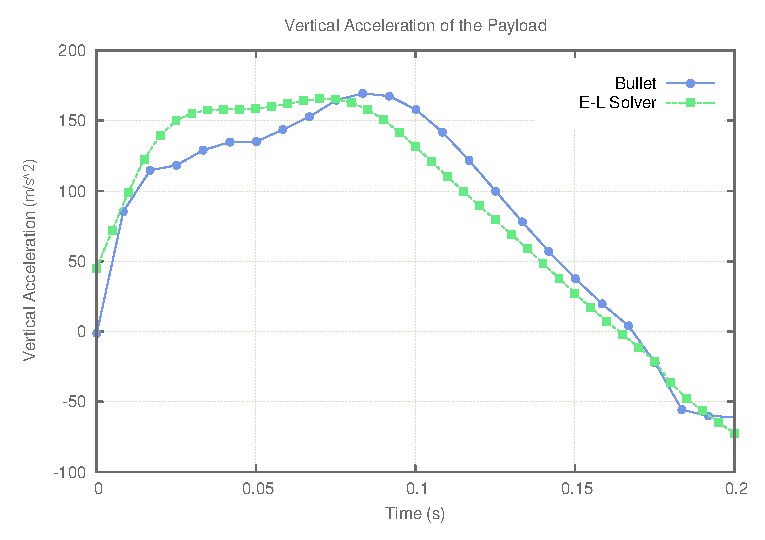
\includegraphics[width=0.8\columnwidth]{tex/images/landing/bulletVsEL/VelocityDerivatives_SimVsEL}
   \caption{NTRT vs EL Vertical Acceleration}
   \label{fig:vsAccelerations}
\end{figure}


\section{Simulated Drop Tests and Payload Protection}

Finally, extensive analysis were performed on  various drop tests and the protection provided to a payload.   As one might expect, varying the rod lengths which impacts the stroke distance for the payload to decelerate, it is possible to control the maximum deceleration experienced by the payload while ensuring that it did not collide with the ground or structure.  For example, with rods of 1.5 meters in length, the payload experienced a max deceleration of 21.4G when landing at 15 m/s. Figure \ref{fig:rodvsG} shows the results of a series of drop tests with different rod lengths and shows the resulting maximum deceleration and forces experienced in the tension members.   As can be seen from these graphs, even for reasonable rod lengths, the maximum G's are acceptable for most instruments, and the maximum forces experienced by the cables are easily within ranges that can be engineered for.  In all tests, the total system mass is kept constant at 100kg (which is 70kg for the payload and 5kg per rod) in order to highlight the impact of structural geometry and rod length.  For the tension members, spring constants of 44 kN/m were used for the cables around the perimeter and 10 kN/m for the cables attached to the payload.  Also, the results in Figure \ref{fig:rodvsG} were found using the landing orientation of 35 degrees around X axis and 45 degrees around Z axis, which were selected from the orientation studies discussed below. 

\begin{figure}[htbp]
\centering
\includegraphics[width=0.8\columnwidth]{tex/images/rodvsG_fixed2}
\caption{{\em {\bf Landing Forces Study}. This shows how rod length impacts maximum deceleration of the payload and  the maximum forces experienced by the tension cables.  All tests were conducted with a landing velocity of 15 m/s onto a hard surface.}}
\label{fig:rodvsG}
\end{figure}

A very interesting point to consider is that the mass of a \SB{} like system will grow in a linear fashion with the length in the rods, while providing increasing payload protection.  On the other hand, the mass of airbags increases with the square of the radius, which is one of the reasons that the MSL rover, with its increased size and mass, had to switch from the airbag approach to the more complex Sky Crane approach.  While this study has focused on small light-weight mission concepts, there could be compelling advantages for scaling up to handle larger payloads.

\section{Landing Orientation Studies}
In order to study how landing orientation affects payload decelerations and impact events, a systematic study of landing orientations was conducted.  In order to get meaningful data, even for bad orientations, a larger tensegrity structure with 4 meter rods was used so the data wouldn't saturate.  The success criteria for this study was that the decelerations had to stay under an upper limit of 25G deceleration of the payload, and the payload had to avoid collision with the ground or parts of the tensegrity structure.  Figure \ref{fig:landingHeatMapRot} shows the orientations that landed safely within these criteria (black) or failed one or both of the criteria (colored).  By using a simple trailing streamer during descent it would be possible to control landing at an optimal orientation and enable the use of smaller structures with shorter rods because the orientation control would maximize the available stroke for the payload to decelerate within the structure.  Conversely, these studies could be used to know what the worst possible landing scenario will be and choose a structure size which will allow safe landing at any orientation.

\begin{figure}[htbp]
   \centering
   \includegraphics[width=0.8\columnwidth]{tex/images/landing/landingHeatMapRot.png}
   \caption{\em Heat map of the maximum acceleration that the payload encounters for all possible landing orientations. Black areas are safe, colored areas are where the payload does not meet one or both success criteria.}
   \label{fig:landingHeatMapRot}
\end{figure}

\section{Conclusions from Simulation Experiments}
Using the scenario of free fall impacts, two different simulation methods were developed and cross-validated which enables the exploration into the capabilities of a tensegrity structure to absorb the forces of landing and to simultaneously protect a delicate payload.  This analysis confirmed that indeed it is possible to do so using a 6-bar tensegrity probe while maintaining maximum decelerations experienced by the instrument-containing payload to forces less than 25G, despite the structure landing at 15 m/s.   Comparing this to the Huygens probe's landing acceleration of \(32G\) \cite{lorenz1994huygens}, the tensegrtiy probe will have a \(43\% \) reduction in \(G\) forces experienced by the scientific payload, despite the Huygens probe's use of parachutes to land at 1/3 of the speed of our tensegrity probe.

\section{Validation of NTRT and Real Hardware Prototypes}
The NASA Tesnsegrity Robotic Toolkit has also been shown to mimic real world robotic prototypes in regards to kinematics and dynamics as well as learning close loop force controls.
Caluwaerts~\etal demonstrated a maximum \(1.3\%\) position error when comparing rod end positions from motion capture data and NTRT~\cite{caluwaerts2014design}. 
For dynamics, they showed less than \(5\%\) time averaged error of each rod end's vertical position in relation of the robot's diameter.
To further validate NTRT, Mirletz~\etal used the simulator to tune Central Pattern Generator (CPG) coupled impedance controllers through Monte Carlo trials~\cite{mirletz2015towards}. 
They were able to demonstrate that there was a maximum error of \(1.6\%\) between the forces seen on their robot vs the forces calculated in the simulator.
%\input{./tex/Results.tex}
%\input{./tex/FutureWork.tex}

% Outline
% Intro about tensegrities. Explain what the structure is and why it is important. Good to mention ideal tensegrities, class system, and prior robots and research.
% Modeling: This section will be a short section on basic linear modeling of a tensegrity structure. Mention that this is not my work, but and explination of prior research. 
% Mechatronics: This will be the longest section. Start off by talking about NIAC and the NASA proposal. Then move to how that directed over arching desgin goals. Move to then talk about the design matrix for SUPERball and how we choose some of the components that we did. Finish by explaining each major portion of the system.
% Results: This section will talk about the itial results from SUPERball. Tension information, motor power and control, battery monitoring, communication (ROS, CAN), 
% Future Work: Talk about where we are taking the project. Movement, learning, etc.

% Bibliography:
\clearpage
\bibliographystyle{plain}
\bibliography{Advancement_Doc_Jonathan_Bruce}

\end{document}
